\begin{enunciado}{\ejercicio}
	Sea $f = X^{68} - 17X^4 - 16 \in \complejos[X]$. Determinar la forma binomial de cada raiz multiple
    de $f$ en $\complejos$ y la multiplicidad de cada una de ellas. 
\end{enunciado}

Primero determinamos las raices multiples, como no voy a factorizar el polinomio pues tiene un grado
muy alto, chequeo las raices de la derivada y veo si coinciden:
$$
 f'(X) = 68X^{67} - 68X^3 \igual{\text{?}} 0 \sii X^3\cdot(X^{64} - 1) = 0 \sii X^3 = 0 \quad \lor \quad X^{64} - 1 = 0
$$
Vemos que $X = 0$ no puede ser pues no es raiz en el original, la otra que nos queda son las raices $64$-avas de la unidad.

Agarro una raiz arbitraria $\omega$ $64$-ava de la unidad distinta de 1, es decir $\omega \neq 1$ y la pruebo en el polinomio:
$$
 f(\omega) = \omega^{68} - 17\omega^4 - 16 = \omega^4 - 17\omega^4 - 16 = -16(\omega^4 + 1) \igual{?} 0 \sii \omega^4 + 1 = 0 \sii \omega^4 = -1.
$$
Obtenemos que las raices son:
$$
 \omega = e^{(\frac{\pi + 2k\pi}{4})i} \quad k = 0,1,2,3
$$
Notar que estas son las raices $8$-avas de la unidad pero que no son $4$-tas. 

Antes de calcular la forma binomial veamos que no hay mas raices de mas multiplicidad. Derivamos la primera derivada:
$$
\begin{array}{rlc}
  f''(X) &= 3X^2\cdot(X^{64} - 1) + X^3\cdot(64X^{63}) \\
  f''(X) &= 3X^{66} - 3X^2 + 64X^{66} = 67X^{66} - 3X^2 \igual{?} 0 \sii 67X^{66} = 3X^2 \sii\\
  &\sii 67X^{64} \igual{$\llamada1$} 3 \sii X^{64} = \frac{3}{67}
\end{array}
$$
En $\llamada1$ se dividió por $X^2$, tomando en cuenta que $X = 0$ es una solucion, sin embargo $0$ no es raiz del polinomio
original. Luego ninguna de las raices van a coincidir con las de la primera derivada. Quedando demostrado que solo tenemos 
raices dobles, procedemos a expresarlas en forma binomial como pide el enunciado.

$$
 \omega = e^{(\frac{\pi + 2k\pi}{4})i} = cos\left(\frac{\pi + 2k\pi}{4}\right) + i sen\left(\frac{\pi + 2k\pi}{4}\right) \quad k = 0,1,2,3
$$
Estos son los puntos que forman angulos de 45 grados en el circulo unitario, ver la figura a continuación:
$$
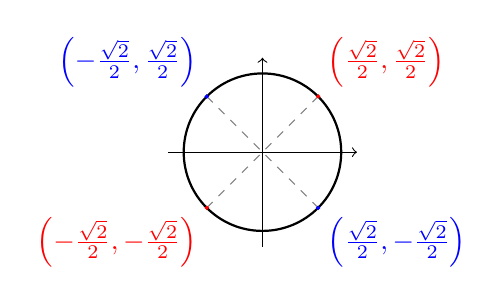
\begin{tikzpicture}[scale=1]
  \draw[->] (-1.2,0) -- (1.2,0) node[right] {};
  \draw[->] (0,-1.2) -- (0,1.2) node[above] {};

  \draw[thick] (0,0) circle(1);

  \draw[dashed,gray] (-0.707,-0.707) -- (0.707,0.707) node[anchor=south west] {};
  \draw[dashed,gray] (-0.707,0.707) -- (0.707,-0.707) node[anchor=north west] {};

  \filldraw[red] ({cos(45)},{sin(45)}) circle(0.02) node[above right] {$\left(\frac{\sqrt{2}}{2}, \frac{\sqrt{2}}{2}\right)$};
  \filldraw[red] ({cos(225)},{sin(225)}) circle(0.02) node[below left] {$\left(-\frac{\sqrt{2}}{2}, -\frac{\sqrt{2}}{2}\right)$};
  \filldraw[blue] ({cos(135)},{sin(135)}) circle(0.02) node[above left] {$\left(-\frac{\sqrt{2}}{2}, \frac{\sqrt{2}}{2}\right)$};
  \filldraw[blue] ({cos(315)},{sin(315)}) circle(0.02) node[below right] {$\left(\frac{\sqrt{2}}{2}, -\frac{\sqrt{2}}{2}\right)$};

\end{tikzpicture}
$$
Finalmente, las formas binomiales de las raices dobles son:
$$
\cajaResultado{
\begin{array}{rcl}
    X_0 &=& \frac{\sqrt{2}}{2} + \frac{\sqrt{2}}{2}i \\
    X_1 &=& -\frac{\sqrt{2}}{2} + \frac{\sqrt{2}}{2}i \\
    X_2 &=& -\frac{\sqrt{2}}{2} - \frac{\sqrt{2}}{2}i \\
    X_3 &=& \frac{\sqrt{2}}{2} - \frac{\sqrt{2}}{2}i \\
\end{array}
}
$$

\begin{aportes}
    \item \aporte{https://github.com/sigfripro}{sigfripro \github}
\end{aportes}